\section{Satisfiability solvers}
\subsection{Propositional Logic}
\begin{itemize}
	\item In Knowledge Representation, we have three sets of rules/formula:
	\begin{itemize}
		\item \textit{Knowledge base}: statements which are known to be true/need to be fulfilled by all models (\textit{axioms})
		\item \textit{Premises}: statements that are only true for certain states/inputs (\textit{implications} at partial truth value assignment)
		\item \textit{Conclusion}: statements for which we want to check if there exists an model for (\textit{conjecture}). Derived by knowledge base and premises
	\end{itemize} 
	\item Propositional logic is based on simple statements (\textit{literals}) that can be combined to complex statements (\textit{formula})
	\begin{itemize}
		\item \textit{Conjunction}: $A\wedge B$
		\item \textit{Disjunction}: $A\vee B$
		\item \textit{Negation}: $\lnot A$
		\item \textit{Implication}: $A\to B$ ($\equiv\lnot A \vee B\equiv \lnot (A \wedge \lnot B)$)
	\end{itemize}
	\item Truth values are assigned to literals by an interpretation function $I$
	\item \textbf{Clausal normal form}
	\begin{itemize}
		\item Every formula can be rewritten in CNF (conjunction of disjunctions)
		\item Example: $(A\vee B\vee C\vee D)\wedge(E\vee F)\wedge(\lnot A \vee F \vee D)\wedge ...$
		\item To rewrite a formula to CNF, we have to remove implications ($A\to B \equiv\lnot A \vee B$), move negations in front of the literals ($\lnot (A\vee B) \equiv \lnot A \wedge \lnot B$) and move conjunctions outside ($A \vee (B\wedge C) \equiv (A\vee B)\wedge (A \vee C)$) 
	\end{itemize}
	\item Propositional logic is a weak language i.e. it is less expressive (no instances, no functions on terms, ...)
	\item We can express first-order logic in propositional logic by instantiating all quantifiers and all possible input arguments to predicates
	\begin{itemize}
		\item Only possible for finite domains. Exponential explosion of number of instances
		\item Example: Domain $\left\{A, B, C\right\}$, $\forall x P(x) \vee Q(x,x)$ $\implies$ $(P\_A \vee Q\_A\_A)\wedge (P\_B \vee Q\_B\_B) \wedge (P\_C \vee Q\_C\_C)$
		\item $\exists x \forall y Q(x, y) \implies (Q\_A\_A \wedge Q\_A\_B \wedge Q\_A\_C) \vee (Q\_B\_A\wedge...)\vee ...$
	\end{itemize}
	\item \textit{Tautology}: formula that is always true (e.g. $A\vee \lnot A$), also called valid sentence. For $n$ symbols, we have $2^n$ models.
	\item \textit{Contradiction}: formula that is always false (e.g. $A\wedge \lnot A$), also called inconsistent sentence
	\item \textit{Satisfiable sentence}: formula that can be made true in at least one world (i.e. not inconsistent)
	\item A \textit{model} is a ``possible world'' (truth assignment) in which the knowledge base is true (including conjecture if given)
	\item $P\models Q$ means that any model of $P$ also fulfills $Q$
\end{itemize}
\subsection{Davis Putman algorithm}
\begin{itemize}
	\item Algorithm for proving if there exists an model for a given knowledge base, \textbf{and} returns it as a result in that case
	\item In general, this problem is NP-complete
	\begin{itemize}
		\item Any other NP problem can be reduced to SAT
		\item Exponential time $\mathcal{O}(2^n)$ with number of literals, but algorithms are optimized to be fast for most cases (only worst case is exponential)
	\end{itemize}
	\item The DPLL algorithm is summarized in Figure~\ref{fig:kr_sat_dpll_algorithm} and described in more detail here:
	\begin{enumerate}
		\item[Step 1] \textbf{Simplification}: iteratively remove unnecessary clauses and derive literal implications
		\begin{itemize}
			\item \textit{Tautology}: remove tautologies like $P\vee \lnot P$ from knowledge base (once in the beginning)
			\item \textit{Pure literals}: set predicates that solely occur in their positive \textit{or} negative form to the corresponding truth value
			\item \textit{Unit clauses}: set literals for which the knowledge base contain a unit clause to true (or the predicate to false respectively)
		\end{itemize}
		\item[Step 2] \textbf{Split}: pick a predicate and assume a truth value
		\begin{itemize}
			\item Heuristics of which literal to pick next can improve the efficiency of DPLL a lot
			\item \textbf{DLCS} (\textit{Dynamic Largest Combined Sum}): Pick $v$ with the largest count of positive and negative occurrences: $CP(v) + CN(v)$. If $CP(v) > CN(v)$, choose $v=1$, else $v=0$
			\item \textbf{DLIS} (\textit{Dynamic Largest Individual Sum}): Pick $v$ with either largest $CP$ or $CN$. Same truth assignment as for \textit{DLCS}.
			\item \textbf{Jeroslow-Wang}: weight of literal depends on the length of clauses it occurs in. Thereby, we prefer small clauses. The score of a literal is $J(v)=\sum_{c\in \mathcal{C}_v} 2^{-|c|}$, and we pick the highest value. One-sided JW looks at $v$ and $\lnot v$ independently, whereas the two-sided approach looks at sum of $v$ and $\lnot v$, and just picks the truth value based on $J(v)\geq J(\lnot v)\Rightarrow v=1$, else $v=0$.
			\item \textbf{MOMs} (\textit{Maximum Occurrences in Clauses of Minimum Size}): similar to JW, but we only look at the smallest clauses in the knowledge base. The number of occurrences in those is indicates by the function $f$. We choose the literal that maximizes $[f(v)+f(\lnot v)]*2^{k}+f(v)\cdot f(\lnot v)$. $k$ is a tuning parameter for the trade-off between the balanced distribution of $v$ and $\lnot v$ and their individual ones.
		\end{itemize}
	\end{enumerate}
	\begin{figure}[ht!]
		\centering
		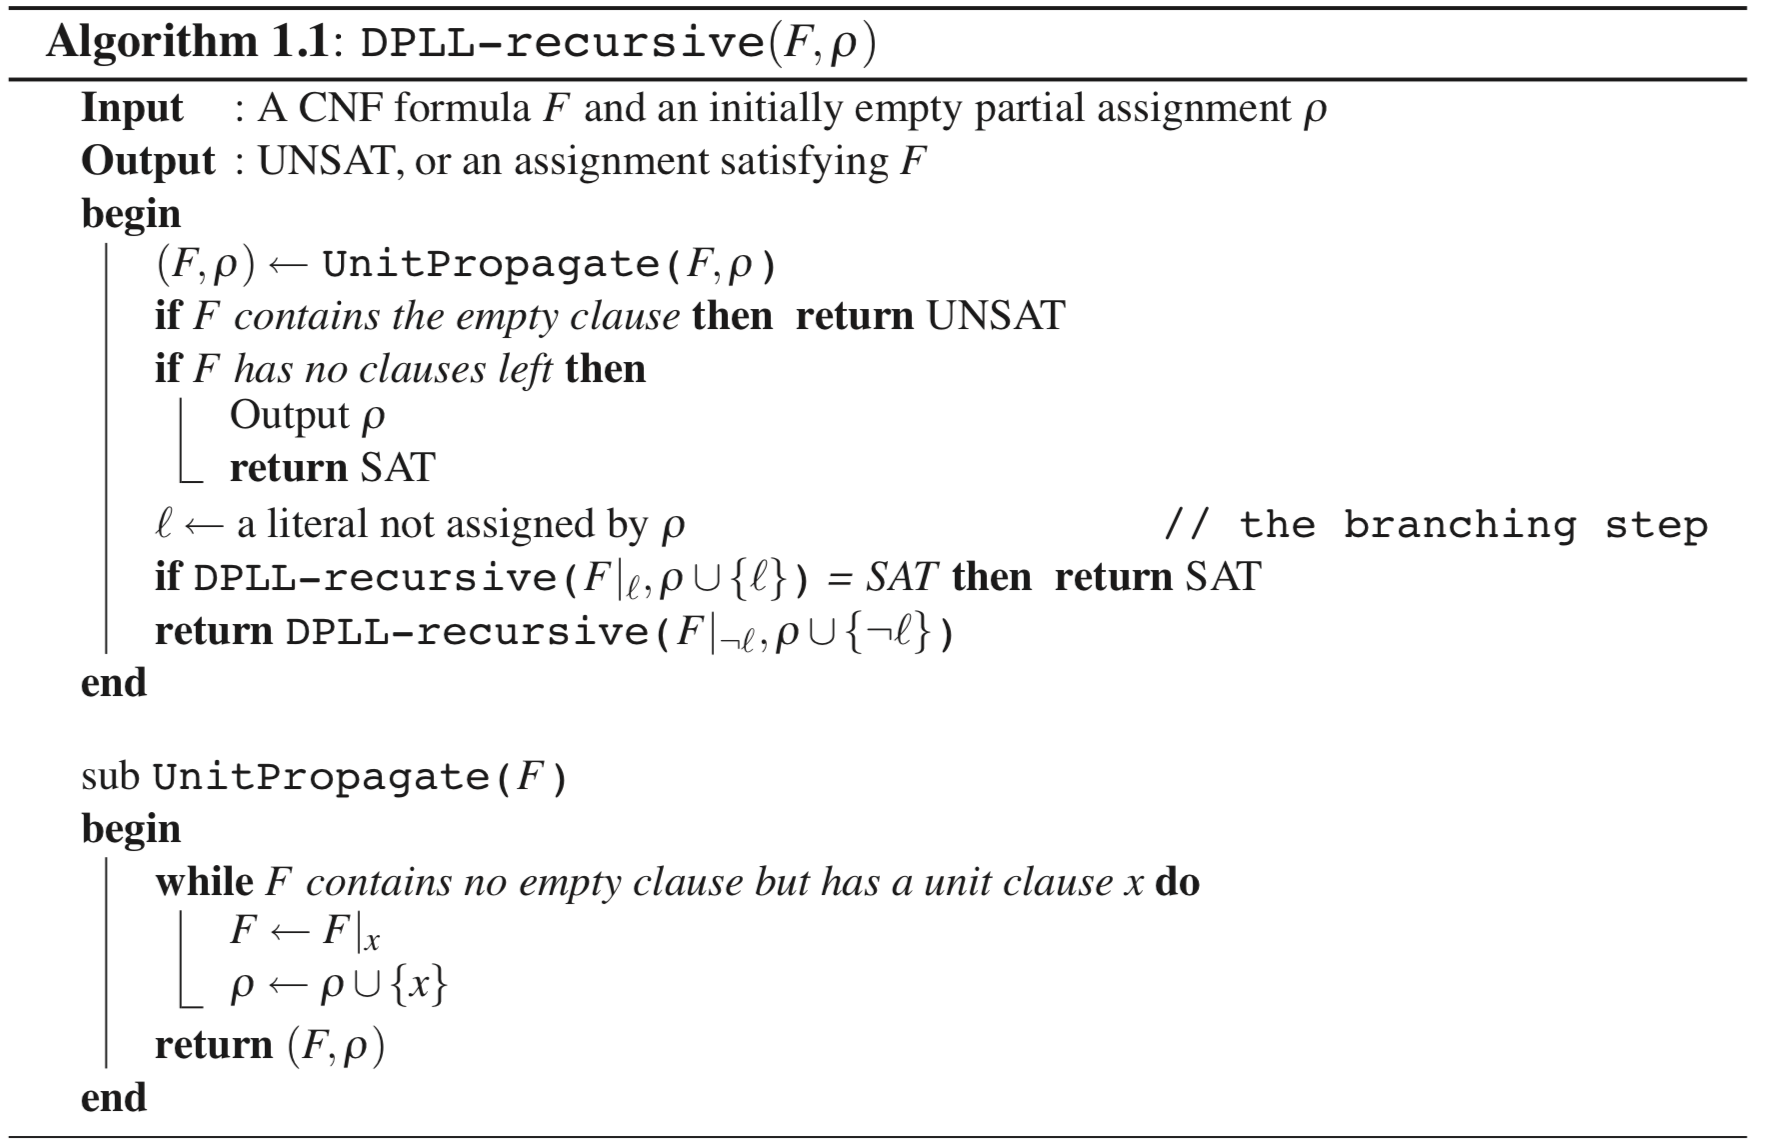
\includegraphics[width=0.6\textwidth]{figures/kr_sat_dpll_algorithm.png}
		\caption{DPLL pseudo-code algorithm}
		\label{fig:kr_sat_dpll_algorithm}
	\end{figure}
\end{itemize}
\subsubsection{Clause Learning}
\begin{itemize}
	\item \textit{Non-chronological backtracking}: If we encounter a conflict at the end of a search branch, we try to find the root of the problem, and then backtrack to the that point.
	\item The implications (decisions/assignments) that lead to a conflict can be modeled as an acyclic graph where each node represents a literal assignment and each edge represents the reason for that assignment (see Figure~\ref{fig:kr_sat_conflict_clause_figure})
	\item We can then partition the graph such that one side contains at least all decision variables (called \textit{reason side}), and the other the conflict literal (called \textit{conflict side}). 
	\item The conflict clause is determined by the negations of the literals associated with the cut between both sides. 
	\item Different cuts of the implication graph distinguish learning schemes from one another as they imply different conflict clauses and hence
	the information gained from them.
	\begin{figure}[ht!]
		\centering
		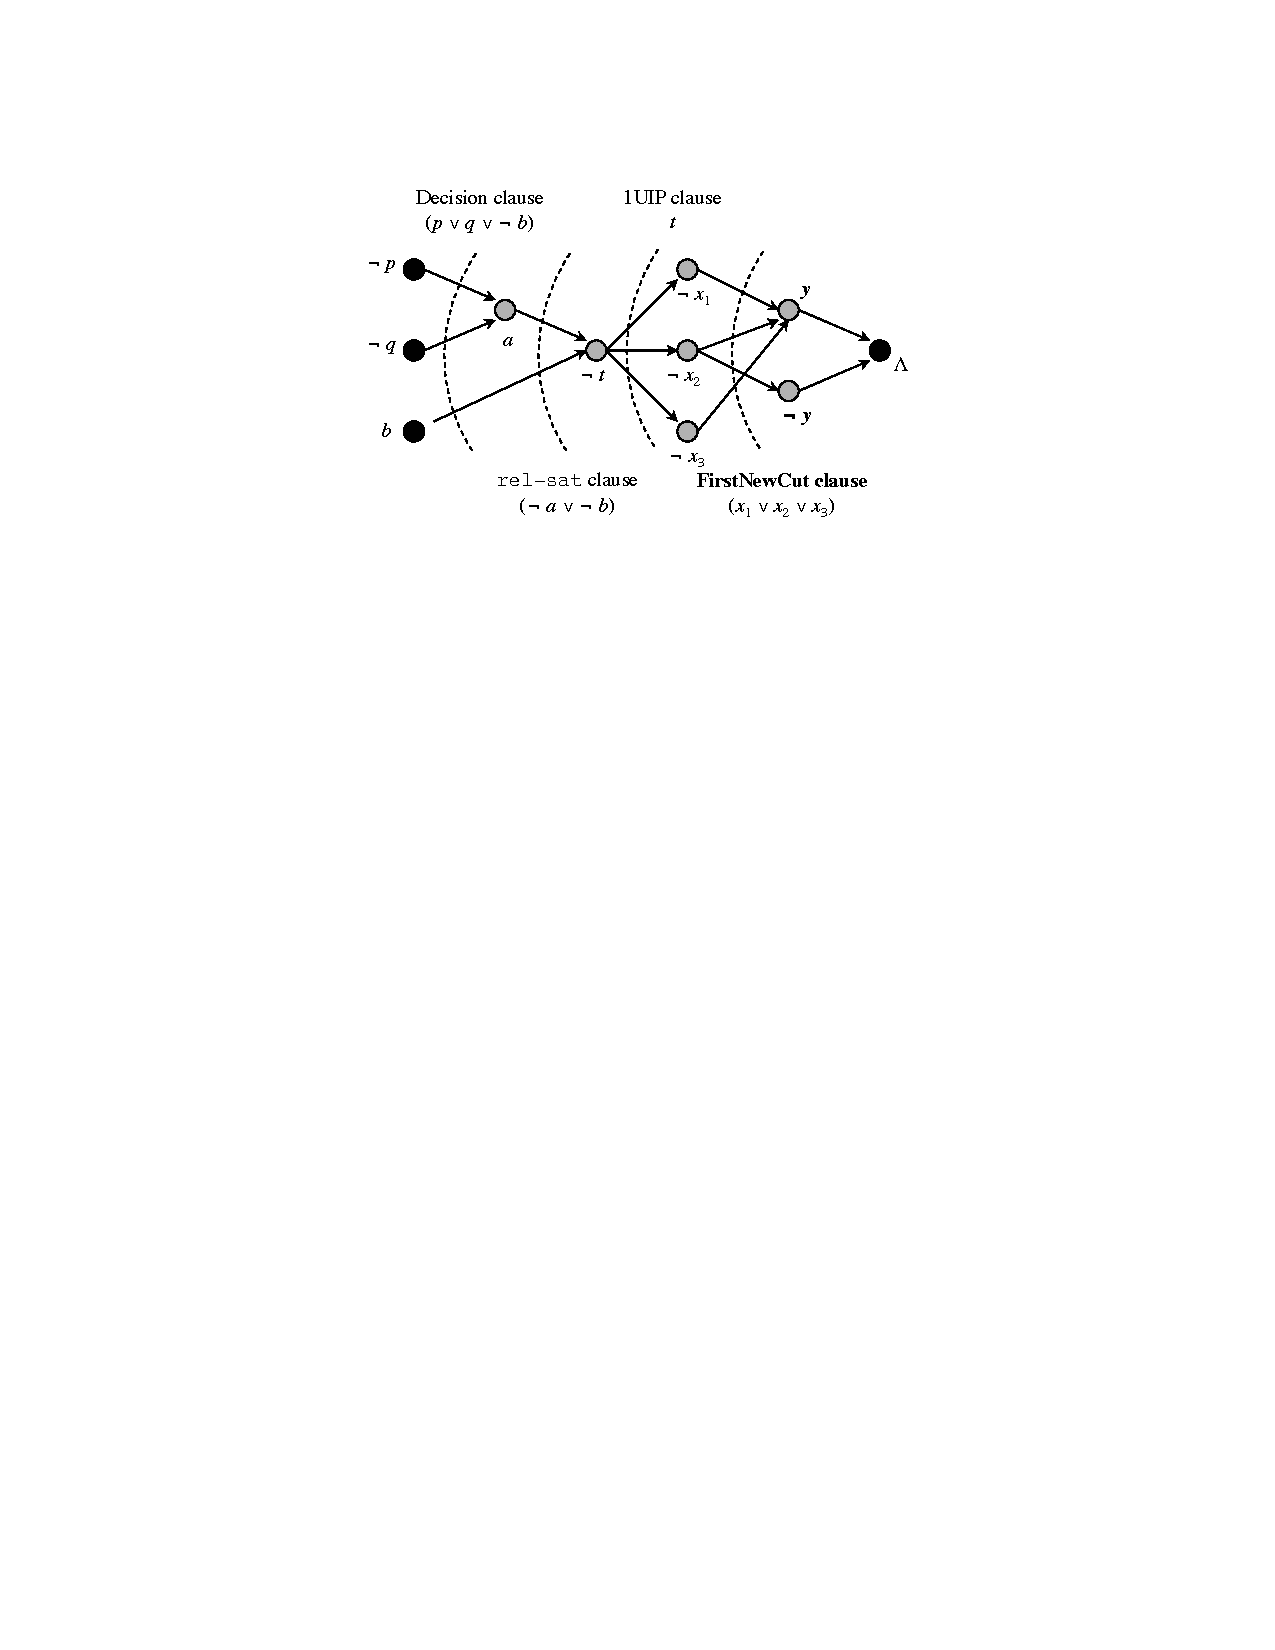
\includegraphics[width=0.3\textwidth]{figures/kr_sat_conflict_clause_figure.pdf}
		\caption{Conflict clause implication graph}
		\label{fig:kr_sat_conflict_clause_figure}
	\end{figure}
	\item Conflict clause learning is a selective application of resolution (probably more useful than random resolution). General resolution rule:
	$$\frac{\hspace{2mm}A\vee \lnot B\hspace{6mm}C\vee B\hspace{2mm}}{A\vee C}$$
\end{itemize}
\subsection{Stochastic solver}
\begin{itemize}
	\item Properties of a SAT solver
	\begin{itemize}
		\item \textit{Decidability} = completeness. 
		\begin{itemize}
			\item This means that given enough runtime, the SAT solver guarantees to find an assignment or returns that there is no solution.
			\item Although DPLL is complete in theory, it is not in practice as we have limited runtime to wait for an answer
			\item Note that \textit{undecidability} just indicates that it is not \textit{always} guaranteed to get an answer (may be harmless in practice)
		\end{itemize}
		\item \textit{Complexity}: exponential maximum runtime $\mathcal{O}(n^2)$
		\begin{itemize}
			\item However, mean instead of worst-case runtime is more important in practice
			\item Also, $\mathcal{O}$-notation does not consider constants whereas with limited runtime, it might be important
			\begin{figure}[ht!]
				\centering
				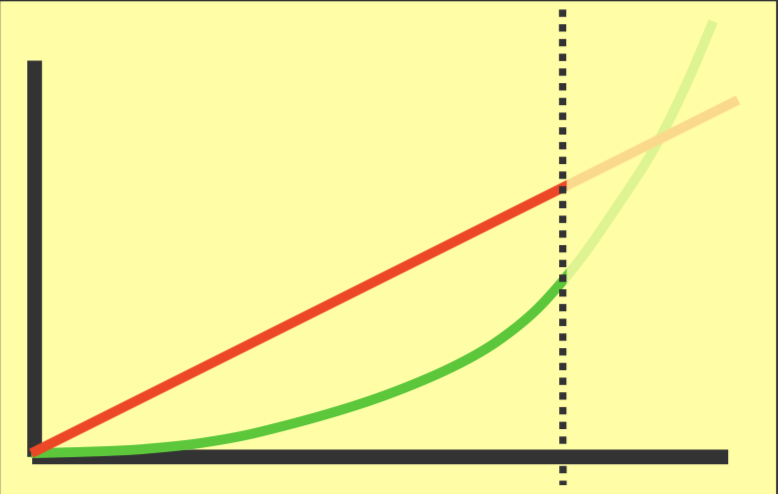
\includegraphics[width=0.2\textwidth]{figures/kr_sat_prob_worst_case.png}
				\caption{Comparison of worst case runtime $\mathcal{O}(n)$ and $\mathcal{O}(n^2)$ with different constants}
				\label{fig:kr_sat_prob_worst_case}
			\end{figure}
		\end{itemize}
	\end{itemize}
	\item A good measurement for complexity in case of SAT solvers has been shown to be the ratio of clauses to variables (see Figure~\ref{fig:kr_sat_prob_hardness})
	\item Problems with a low ratio are easy to solve as they have (in average) many solutions
	\item Problems with a high ratio tend to have no solution, and are easy to show that there exists a conflict (see Figure~\ref{fig:kr_sat_prob_hardness_2})
	\item In between, around $4.26$, are apparently the hardest randomly generated problems as there might a solution (or only a few) or not. This points is also referred to as \textit{phase transition}
	\begin{figure}[ht!]
		\centering
		\begin{subfigure}[b]{0.23\textwidth}
			\centering
			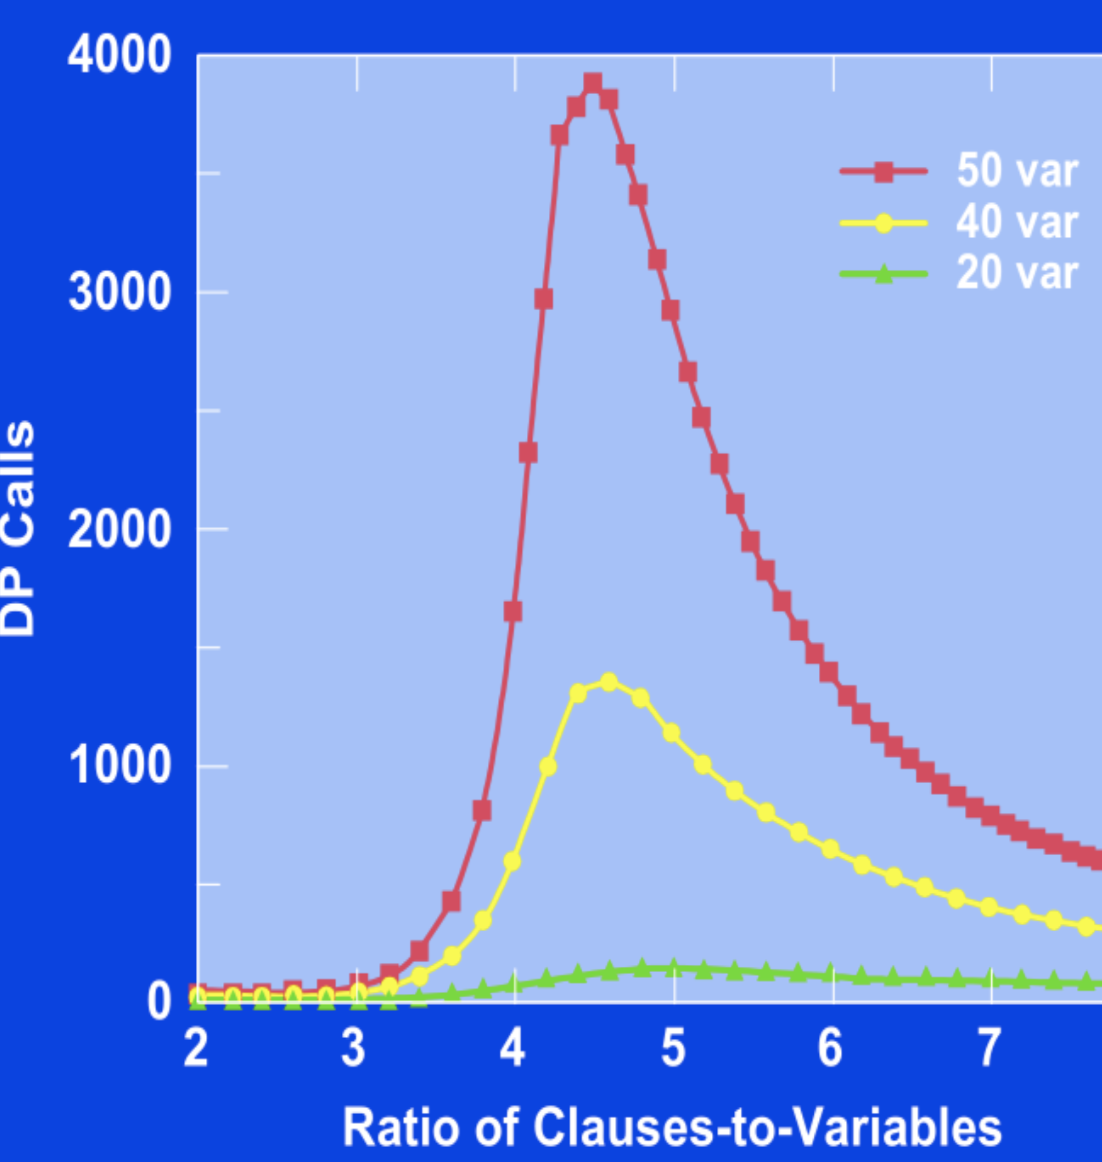
\includegraphics[width=\textwidth]{figures/kr_sat_prob_hardness.png}
			\caption{Problem complexity}
		\end{subfigure}
		\hspace{10mm}
		\begin{subfigure}[b]{0.4\textwidth}
			\centering
			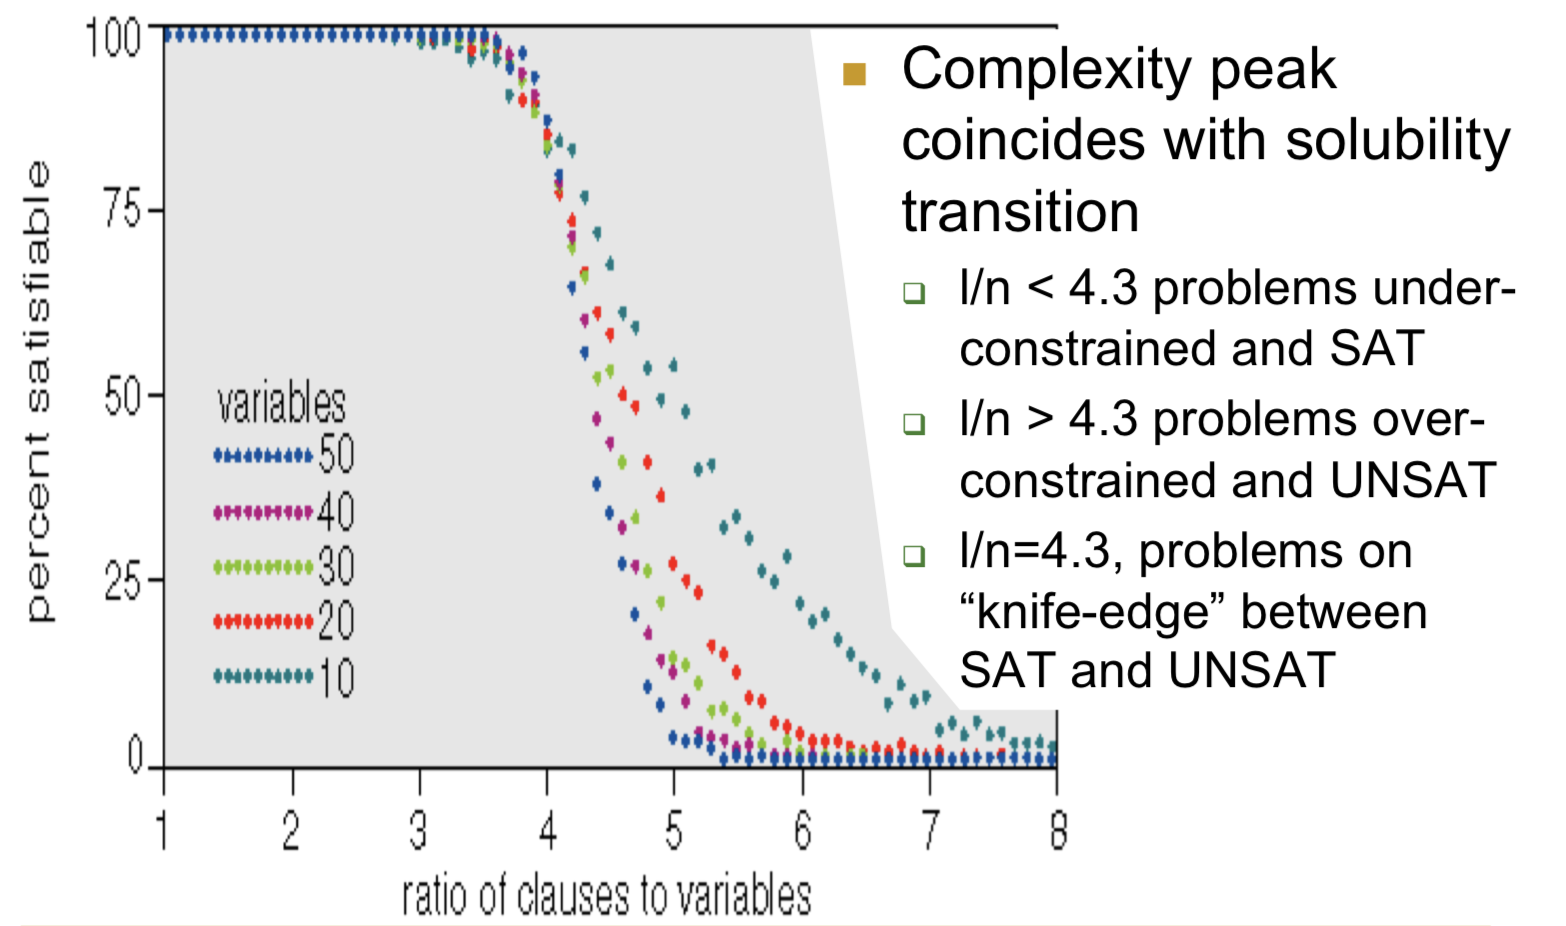
\includegraphics[width=\textwidth]{figures/kr_sat_prob_hardness_2.png}
			\caption{Proportion of satisfiable problems}
			\label{fig:kr_sat_prob_hardness_2}
		\end{subfigure}
		\caption{Hardness in SAT problems}
		\label{fig:kr_sat_prob_hardness}
	\end{figure}
	\item Stochastic solvers have been shown to perform quite well on such randomly generated SAT instances, but might perform poorly compared to DPLL on highly structured problems
	\item It is not intended to find all solution neither that there exists none. But is for example useful for MAXSAT (see later)
	\item Stochastic SAT solvers perform local search 
	\begin{enumerate}
		\item Make a guess (smart or random) about values of the variables
		\item Evaluate how many clauses are broken
		\item Try flipping a variable to make things better for a certain number of iterations (various heuristics in which variables to flip next)
	\end{enumerate}
	\item This search is repeated $N$ times until we either find a solution or terminate without an answer
	\item \textbf{GSAT}: Local greedy search/algorithm of picking the next variable to flip which increases the number of satisfied clauses the most (ties are broken randomly, note that flips will break also some clauses).
	\item Full algorithm shown in Figure~\ref{fig:kr_sat_prob_GSAT}
	\item Note that this algorithm tends to get stuck in local minimum (flipping a single variable does not increase score). Thus, we perform random restarts to start new. That's also why GSAT spends most time on plateaus where score is not improved
	\begin{figure}[ht!]
		\centering
		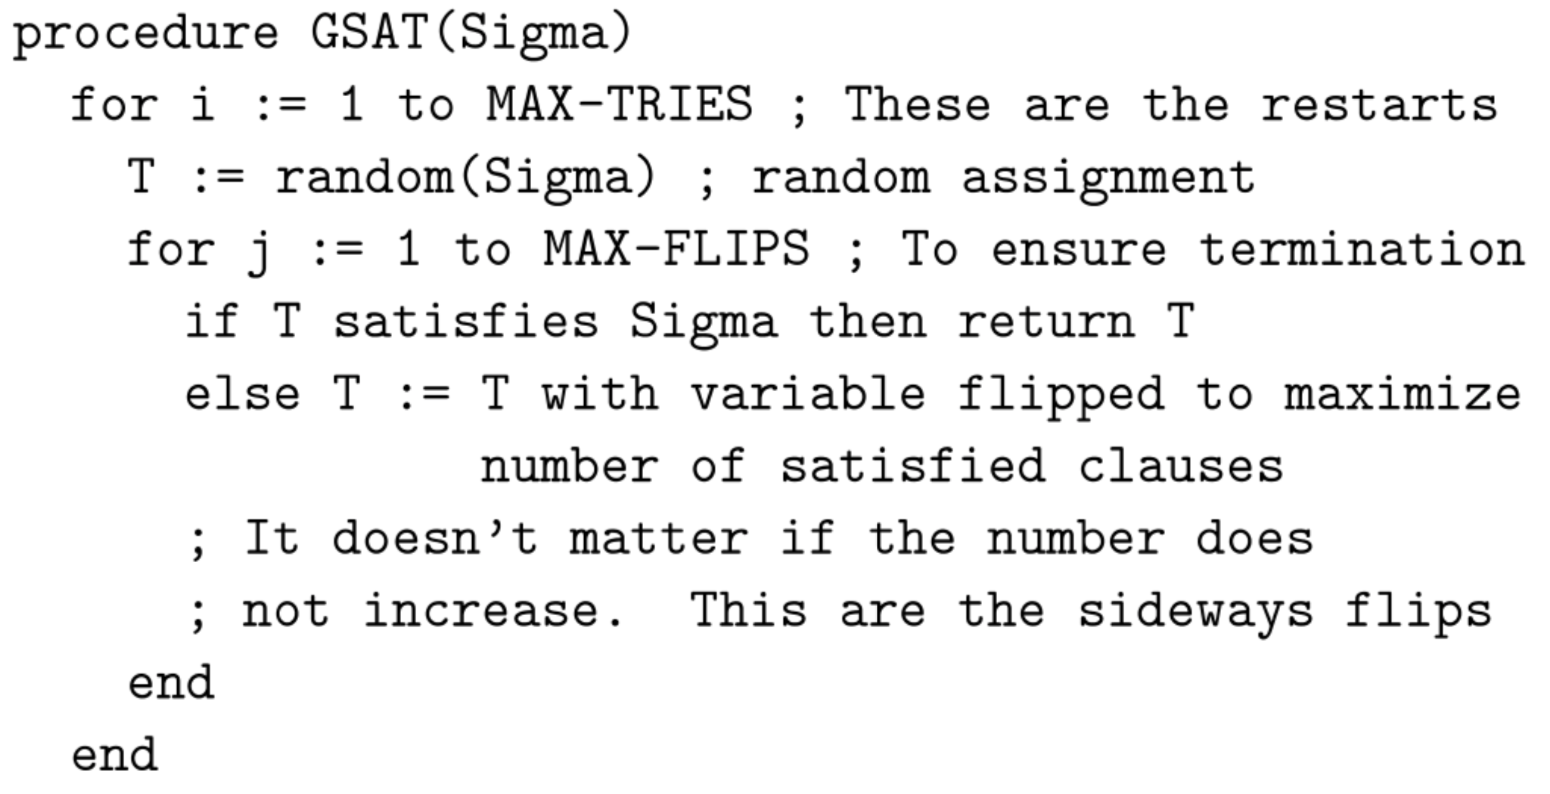
\includegraphics[width=0.5\textwidth]{figures/kr_sat_prob_GSAT.png}
		\caption{Pseudo-code of GSAT}
		\label{fig:kr_sat_prob_GSAT}
	\end{figure}
\end{itemize}
\subsection{MAXSAT}
\begin{itemize}
	\item MAXSAT is Proportion \textit{optimization} extension of SAT that asks what is the maximum number of clauses that can be simultaneously satisfied
	\item Example: $\lnot A\wedge (A \vee B) \wedge (\lnot B)$ is a contradiction. But the truth assignment $\pi = \left\{\lnot A, \lnot B\right\}$ maximizes number of satisfied clauses
	\item Some clauses might be more important to be satisfied than others $\Rightarrow$ adding a cost/positive weight to every clause $C$ that will be incurred if $C$ is falsified
	\item A cost of $\infty$ indicates \textit{hard} clauses that are mandatory to satisfy, whereas \textit{soft} clauses have a finite cost
	\item We try to minimize the sum of the costs of all unsatisfied clauses
	\item There are different variations of MAXSAT:
	\begin{itemize}
		\item (Standard) MAXSAT: no hard clauses and all have a weight of 1 (solution maximizes the number of satisfied clauses)
		\item \textit{Weighted} MAXSAT: no hard clauses, but soft clauses with any finite, positive weight
		\item \textit{Partial} MAXSAT: hard clauses are allowed, but all soft clauses have weight 1
		\item \textit{Weighted Partial} MAXSAT: both hard and soft clauses are allowed. Subsumes all previously mentioned variations.
	\end{itemize}
\end{itemize}
\subsection{SAT planning}
\begin{itemize}
	\item Real-world planning problems can be translated to a SAT problem, and the plan can be extracted from the truth assignments\\
	\begin{minipage}{.65\textwidth}
		\item Formal definition of the planning problem
	\begin{itemize}
		\item States $S=\left\{...,s_i,...\right\}$ (in the example $S=\left\{s_0, s_1, s_2, s_3, s_4, s_5\right\}$)
		\item Actions $A=\left\{..., a_i,...\right\}$ (in the example $A=\left\{\texttt{move1}, \texttt{move2}, \texttt{put}, \texttt{take}, \texttt{load}, \texttt{unload}\right\}$)
		\item State-transition function $\gamma:S\times A\to S$ (note that we only consider deterministic transitions, otherwise $2^S$ output)
		\item Planning problem $P=(\Sigma, s_0, s_G)$ where $\Sigma=(S,A,\gamma)$, and $s_0$ initial state and $s_G$ (set of) goal states
		\item Classical plan is a sequence of actions: $\pi = \langle a_0, a_1, ..., a_{n-1}\rangle$
		\item Policy is a partial function from $S$ to $A$
	\end{itemize}
	\end{minipage}
	\hspace{10mm}
	\begin{minipage}{.3\textwidth}
			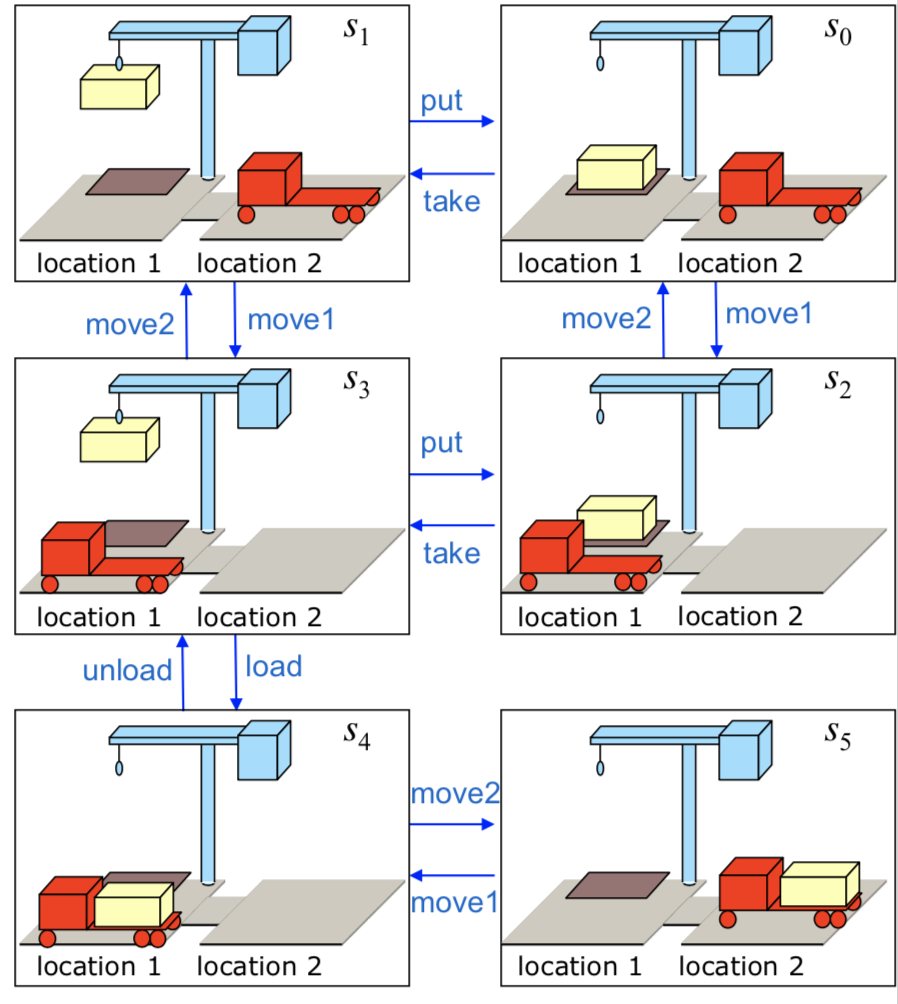
\includegraphics[width=0.8\textwidth]{figures/kr_sat_planning_example.png}
			\label{fig:kr_sat_planning_example}    
	\end{minipage}
	\item Translation for plan $P$ and a fixed plan length $n$:
	\begin{itemize}
		\item If $\pi=\langle a_0, a_1, ..., a_{n-1}\rangle$ is a solution to the planning problem, we know that the traversed states are $s_0, s_1 = \gamma(s_0, a_0), s_2 = \gamma(s_1, a_1), ..., s_n = \gamma(s_{n-1}, a_{n-1})$ (where $a_i$ is the $i$-th step of $\pi$, and $s_i$ the states in which the agent is at step $i$)
		\item We denote all possible literals with $L$
		\item Formula describing the initial state: $\bigwedge\left\{l_0\hspace{1mm}|\hspace{1mm}l \in s_0\right\} \wedge \bigwedge\left\{\lnot l_0\hspace{1mm}|\hspace{1mm}l \in L-s_0\right\}$
		\item Formula describing the goal state: $\bigwedge\left\{l_n\hspace{1mm}|\hspace{1mm}l \in g^+\right\} \wedge \bigwedge\left\{\lnot l_n\hspace{1mm}|\hspace{1mm}l \in g^{-}\right\}$ ($g^{+}$ valid goal states, $g^{-}$ invalid goal states)
		\item Formula describing the state-transitions. For every $a_i$ add $\bigwedge\left\{p_i\hspace{1mm}|\hspace{1mm}p\in \text{Precond}(a)\right\} \wedge \bigwedge\left\{e_{i+1}\hspace{1mm}|\hspace{1mm}e\in \text{Effects}(a)\right\}$
		\item Complete exclusion axiom: only one action per step ($\lnot a_{1,i} \vee a_{2,i}$,...)
		\item Frame axioms that describe what \textit{doesn't} change between $i$ and $i+1$: $\left(\lnot l_i \wedge l_{i+1} \Rightarrow \bigvee_{a\in A} \left\{ a_i | l \in \text{Effects}^+ (a) \right\} \right) \wedge \left(l_i \wedge \lnot l_{i+1} \Rightarrow \bigvee_{a\in A} \left\{ a_i | l \in \text{Effects}^- (a) \right\} \right)$ ($\text{Effects}^+ (a)$: set of literals that change their truth value to true if $a$ is performed, and $\text{Effects}^- (a)$ those that are changed to false)
	\end{itemize}
	\item We apply a SAT solver on this knowledge base. If we find a solution, then $P$ has a solution of length $n$
	\item To find solutions of shortest length, we loop over different values for $n$. If we don't find any solution for $n=0$, we encode the problem for $n=1$, and so on.
	\item In practice, SAT solvers for planning take too much time and memory, but can be combined with other techniques like planning-graph expansion (SatPlan).
\end{itemize}
\subsection{Applications of SAT}
\begin{itemize}
	\item Model checking in terms of hardware and software verification (can state $S$ be ever reached? Is state $T$ always reached after $S$?)
	\item Classical planning
	\item Combinatorial design (existence of mathematical structures)
	\item Solving subproblems in domains like scheduling, test pattern generation, multi-agent systems, ...
\end{itemize}